%!TEX root = ClementiCooperBarba2018.tex

\subsection{Isolated nanoparticle} \label{sec:verification}

In this section we present the results of performing a verification exercise. We
compare our numerical calculations of the extinction cross-section using boundary
elements method (BEM), with analytical solutions available for spherical geometries. 

The analytical expression for the extinction cross-section of spherical geometries
provided by Mishenko \cite{Mishchenko2007} applies for all mediums. In the presence
of a lossy medium, $k^\prime$ represents the real part of the complex wave number,
otherwise $k$ is a real-valued and we take $k^\prime = k$. 


\begin{equation} 
    C_\text{ext} = \frac{4\pi a^3}{k^\prime} \operatorname{Im}\left(k^2 
                    \frac{\epsilon_p/\epsilon_m -1}{\epsilon_p/\epsilon_m +2}\right)
    \label{eq:an_sol}
\end{equation}

where $a$ is the radius of the sphere, $k$ the complex wave number ($k=k^\prime +i k^{\prime\prime}$), $\epsilon_p$ 
the dielectric constant of the particle, and $\epsilon_m$ the dielectric constant
of the host medium. 

When we applied the electrostatic approximation, the simulation reduces to a 
sphere under a constant electric field, like presented in Fig. \ref{fig:np_elec_field}.

\begin{figure}[h] %  figure placement: here, top, bottom, or page
   \centering
   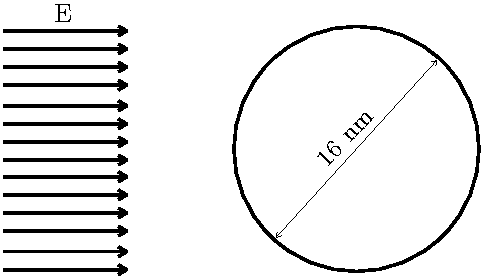
\includegraphics[width=0.3\textwidth]{sphere_field_8nm.pdf} 
   \caption{Spherical nanoparticle in a constant electric field.}
   \label{fig:np_elec_field}
\end{figure}

Figure \ref{fig:error_sphere_Ag} shows a grid convergence study of the extinction
cross-section of a silver spherical nanoparticle of radius $8 \, nm$ immersed in water
under a z-polarized electric field with a wavelength of $380 nm$ and intensity of 
$-0.0037 e/({\AA}^2 \, \epsilon_0)$. Under these conditions water has a dielectric
constant of $1.7972 \, + \, 8.5048^{-09}i$ \cite{JohnsonChristy1972} and silver of
$-3.3877 \, + \, 0.1922i$ \cite{HaleQuerry1972}. In these simulations we used $K=4$ 
Gauss quadrature points per far-away elements, $K_{fine} = 37$ Gauss quadrature points
per elements for near singular integrals, $Nk = 9$ Gauss quadrature points per 
triangle edge for semi-analytical integration in the singular elements, $P=15$ for 
the order of expansion in treecode, and a GMRES tolerance of $10^{-5}$. We
performed the simulation for meshes of 512, 2048, 8192 and 32768 elements. The 
error calculation uses the analytical solution $C_{ext} = 1854.4765 \; nm^2$ 
obtained using equation \eqref{eq:an_sol}.

\begin{figure}[h] %  figure placement: here, top, bottom, or page
   \centering
   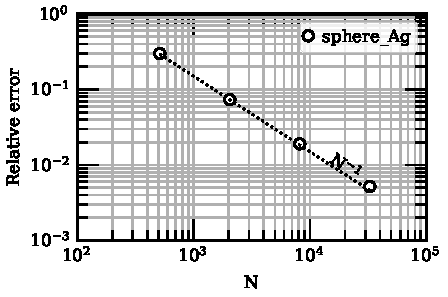
\includegraphics[width=0.45\textwidth]{convergence_sph_Ag_R8_w=380.pdf} 
   \caption{Grid-convergence study of extinction cross-section of a spherical silver
            nanoparticle.}
   \label{fig:error_sphere_Ag}
\end{figure}

The computed order of convergence is $0.98$ and the $1/N$ slope in Fig.\ref{fig:error_sphere_Ag}
shows that the numerical solutions computed with \pygbe for isolated spheres are
correctly resolved by the meshes.

The percentage errors for the different meshes are presented in Table. \ref{table:err_iso_sphere}.

\begin{table}[h]
    \centering
    \caption{\label{table:err_iso_sphere} Percentage error of isolated silver sphere.} 
    \begin{tabular}{c c}
    \hline%\toprule
    N & \% error \\
    \hline%\midrule
     $512$ & $29.86$ \\
     $2048$ & $7.33$ \\
     $8192$ & $1.9$ \\
     $32768$ & $0.52$ \\
    \hline%\bottomrule
    \end{tabular}
\end{table}


To complete the process of verification we performed simulations of the extinction 
cross-section of the isolated sphere for a spectrum of wavelengths. To ensure 
errors $<2\%$ we use the mesh of $N=32768$ elements. 

Figure \ref{fig:verif_sphere} shows the extinction cross-section of the isolated
sphere of Fig.\ref{fig:np_elec_field} as a function of the wavelength. The values of 
the dielectric constants for each wavelength were obtained by interpolation of 
experimental data \cite{JohnsonChristy1972, HaleQuerry1972}. \textcolor{red}{(see how to add
reference to notebooks that generate these values)}


\begin{figure}[h] %  figure placement: here, top, bottom, or page
   \centering
   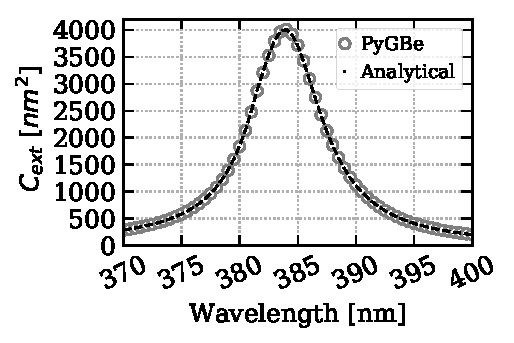
\includegraphics[width=0.45\textwidth]{silver_NP_verification.pdf} 
   \caption{Extinction cross-section as a function of wavelength for a $8 \, nm$
            silver sphere immersed in water.}
   \label{fig:verif_sphere}
\end{figure}

We can see good agreement between simulations and analytical results, proving
that we are achieving an accurate numerical solution of the mathematical model. The 
peak in the extinction cross-section indicates that the plasmons of the metallic
nanoparticle are resonating with the incoming electric field.


\subsection{LSPR response to BSA} \label{sec:lspr_response}

Localized Surface Plasmon Resonance biosensors detect a target molecule by monitoring
plasmon resonance frequency changes due to the proximity of the target to the metallic
nanoparticle. In this section we perform simulations that show how our BEM approach
can be used to model the response of LSPR biosensors.

To ensure that we are achieving an accurate numerical solution, we did a grid 
convergence analysis of the system showed in Figure \ref{fig:setup_conv} . Where
we used as analyte a Bovine Serum Albumina (PDB code 4FS5) protein. The BSA mesh
was generated using the open source software Nanoshaper \textcolor{red}{(missing how to cite - not
reported in their webpage)}. Nanoshaper takes as input the coordinates and radius
of the atoms in the crystal structure, which were extracted from the the van der
Waals radii and charges of the atoms file (\texttt{pqr}) generated using 
\texttt{pdb2pqr} \cite{Dolinsky04}, with the built-in \texttt{amber} force field.

Since we compute the extinction cross section over the sphere nanoparticle, we 
set a fixed mesh density for the protein and refined the mesh of the
sphere (meshes of 512, 2048, 8192 and 32768 elements). After studying different 
cases we decided to use a mesh of density of two triangles per ${\AA}^2$ for 
the protein, resulting in $N_{prot} = 98116$ elements. 


\begin{figure}[h] %  figure placement: here, top, bottom, or page
   \centering
   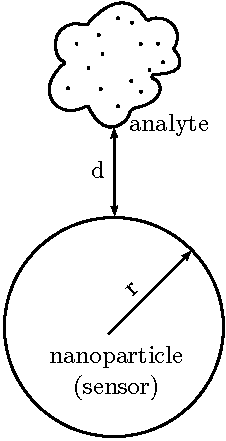
\includegraphics[width=0.15\textwidth]{protein_sphere_sketch.pdf} 
   \caption{Setup for convergence analysis of the response calculation.}
   \label{fig:setup_conv}
\end{figure}

We repeated the conditions and parameters for the isolated sphere simulation
presented in Section \ref{sec:verification}. In this case we added the 
dielectric constant of the protein $2.7514 + 0.2860i$ extracted from the 
functional relationship provided by Pahn, et al. \cite{PahnETal2013}, and the 
distance between the sensor and the analyte was $d=1 \, nm$.  The dipole moment 
of the protein was aligned with the y-axis. The error calculations
use the Richardson extrapolation value of the extinction cross-section as a
reference, $C_{ext}= 1778.7259 \, nm^2$


\begin{figure}[h] %  figure placement: here, top, bottom, or page
   \centering
   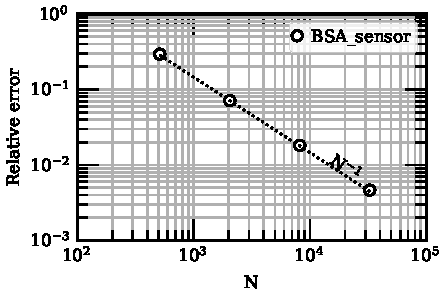
\includegraphics[width=0.45\textwidth]{convergence_bsa_sensor_R8_d=1_w=380.pdf} 
   \caption{Grid-convergence study of extinction cross-section of a spherical silver
            nanoparticle with a BSA protein at $d=1 \, nm$.}
   \label{fig:error_sphere-bsa}
\end{figure}

The computed order of convergence is $0.99$, and we can see in 
Figure \ref{fig:error_sphere-bsa} that the error decays with the number
of boundary elements ($1/N$), which is consistent with our verification 
results of Section \ref{sec:verification}. This proves that the
numerical solutions computed with \pygbe are correctly resolved by the meshes.

The percentage errors for the different meshes are presented in Table. \ref{table:err_bsa_sensor}.

\begin{table}[h]
    \centering
    \caption{\label{table:err_bsa_sensor} Percentage error of BSA-sensor sytem (Fig.\ref{fig:setup_conv}) .} 
    \begin{tabular}{c c}
    \hline%\toprule
    N & \% error \\
    \hline%\midrule
     $512$ & $29.39$ \\
     $2048$ & $7.13$ \\
     $8192$ & $1.82$ \\
     $32768$ & $0.46$ \\
    \hline%\bottomrule
    \end{tabular}
\end{table}

We performed a relaxation of parameters study before we computed the LSPR 
response to the BSA protein. To optimize run time without compromising our small
percentage error, we reduced the density of the protein mesh to one element per
${\AA}^2$ ($N_{prot}=45140$) and fixed the sphere mesh to $N_{sensor}=32768$. We
set $K=4$ Gauss quadrature points per far-away elements, $K_{fine} = 19$ Gauss
quadrature points per elements for near singular integrals, $Nk = 9$ Gauss 
quadrature points per triangle edge for semi-analytical integration in the 
singular elements, $P=6$ for the order of expansion in treecode, and a GMRES 
tolerance of $10^{-3}$. These choices result in a percentage error of $\sim\%0.6$
and the time of each computation is approximately $7.5 min$ in a \texttt{NVIDIA Tesla K40 GPU}
card. 

We studied the LSPR response as a function of the wavelength in the presence 
of the BSA. We run simulations on the system presented in Figure 
\ref{fig:display_z}. As you can see we used two BSA located at $d=1 \, nm$ of distance
along the z-axis. By using two proteins we can appreciate better the effect 
of the BSA. The distance between two wavelengths points is $0.25 \, nm$ and the 
range explored goes from $382 \, nm$ to $387 \, nm$, giving a total of 21 
wavelength points. The location of $+z$ protein is the same used for converge 
analysis, while the protein in the $-z$  position was located there by performing
a solid rotation respect to y-axis of the $+z$ BSA. 


Figure \ref{fig:2pz_response} shows the variation of the extinction cross-section
with respect to wavelength in a near-range around the resonance peak. We can observe
that there is a red-shift ($0.5 \, nm$) in the resonance frequency due to the
presence of the BSA analytes. This result agrees with experimental observations
\cite{TangETal2010, RaphaelETal2013}. Particularly, we observed a decrement of 
the peak which is also present in the results of Tang, et al. \cite{TangETal2010}.
Both results, the red-shift and the decrement of the peak in the presence of 
the proteins, indicate that our boundary element method approach using electrostatic
approximation, is capable of reproducing the characteristic resonance frequency 
shift in LSPR biosensors.


\begin{figure}[h] %  figure placement: here, top, bottom, or page
   \centering
    %since we have dots in the names we need to enclose what is before the 
    %extension in { }
   \includegraphics[width=0.45\textwidth]{{2pz_00_ef-0.0037_R8nm}.pdf} 
   \caption{Extinction cross-section as a function of wavelength for a $8 \, nm$
            silver sphere immersed in water with two BSA proteins placed at
            $\pm 1 \; nm$ away from the surface in the z-direction, and at
            infinity (no protein).}
   \label{fig:2pz_response}
\end{figure}


To study the effect of location of the analytes, we rearange them in 
different locations and run the simulation with the same parameters used before. 
We studied two different cases, one with the analytes located at $\pm 1 \; nm$
of the surface along x-axis, and the other along the y-axis. See Figure \ref{fig:display_xy}
to visualize displays.


Figure \ref{fig:2pxy_response} show the results obtained for x-axis and
y-axis display, respectively. 

\begin{figure}[!h] %  figure placement: here, top, bottom, or page
   \centering
   \subfloat{\includegraphics[width=0.45\textwidth]{{2px_00_ef-0.0037_R8nm}.pdf}}
   \quad 
   \subfloat{\includegraphics[width=0.45\textwidth]{{2py_00_ef-0.0037_R8nm}.pdf}} 
   \caption{Extinction cross-section as a function of wavelength for a $8 \, nm$
            silver sphere immersed in water with two BSA proteins placed at
            $\pm 1 \; nm$ away from the surface in the x-direction (top) and
             y-direction (bottom), and at infinity (no protein).}
   \label{fig:2pxy_response}
\end{figure}

In both cases we can observe that the shift is negligible. According to 
calculations, the shift is smaller than the distance between two wavelengths 
points ($< 0.25 nm $) which results in zero-shift. These findings are consistent with 
the fact that we have a z-polarized electric field. Having a z-polarized electric
field implies that the cloud of electrons will be smaller in the x and y direction.
Therefore, the effect of the analyte in those locations results insignificant. 


Experiments suggests that the distance between the nanoparticle and the analyte 
affects the sensitivity of the sensor \cite{HaesETal2004}. The sensitivity of 
the biosensor is the relation between the size of the shift and the number of 
analytes bound to the ligand molecule. Figure \ref{fig:dist_response} shows how
the peak varies with the distance at which the analytes are placed.  


\begin{figure}[h] %  figure placement: here, top, bottom, or page
   \centering
   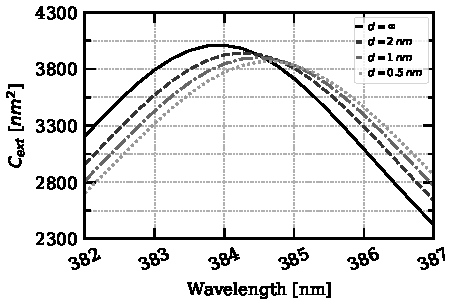
\includegraphics[width=0.45\textwidth]{2pz_lspr_response.pdf} 
   \caption{Extinction cross-section as a function of wavelength for a $8 \, nm$
            silver sphere immersed in water with two BSA proteins placed at
            $2, \, 1 \, \text{and} \, 0.5 \, nm$ away from the surface in the 
            z-direction, and at infinity (no protein)}
   \label{fig:dist_response}
\end{figure}

We can observe how the sensitivity is affected by the distance between the 
analyte and the sensor: the closest they are, the larger the shift. In this particular
case we go from a shift of $0.25 \, nm$ when $d=2 nm$ to $0.75 nm$ when the 
analytes are placed at $d=0.5 \, nm$. This result shows the potential of \pygbe 
and the electrostatic approach to study sensitivity versus distance.

\begin{figure*}[] %  figure placement: here, top, bottom, or page
   \centering
   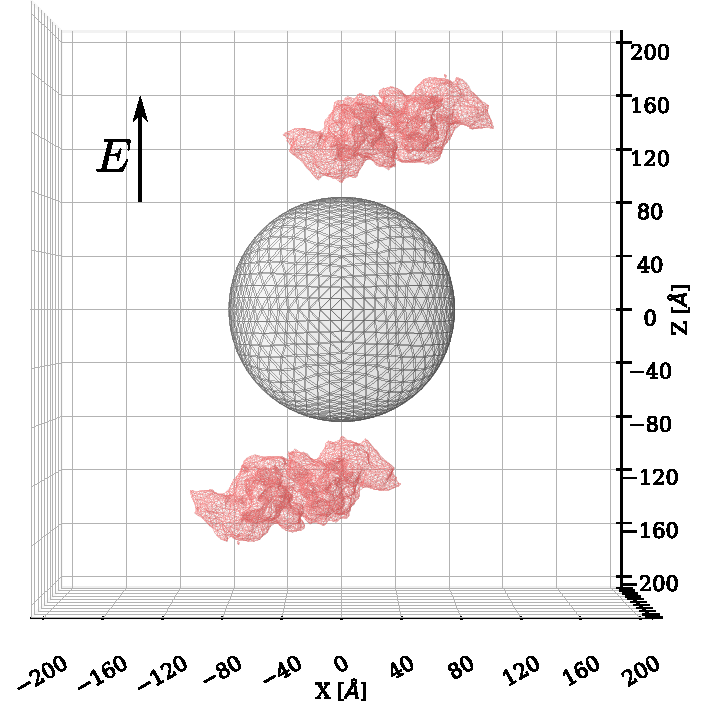
\includegraphics[width=0.65\textwidth]{2prot_1nm_z_R8nm.pdf} 
   \caption{Sensor protein display: BSA located at $\pm 1 \, nm$ of the 
            nanoparticle in the z-direction}
   \label{fig:display_z}
\end{figure*}

\begin{figure*}[]

   \centering
   \subfloat{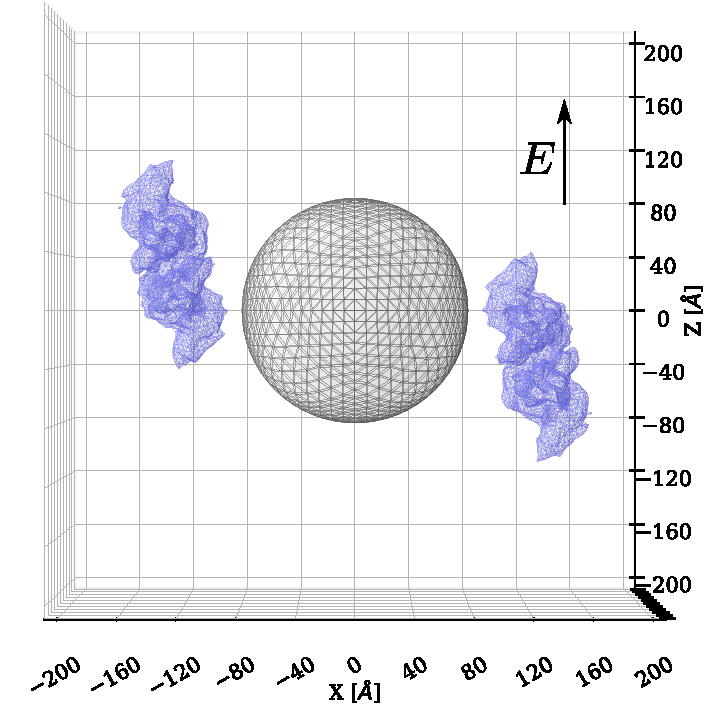
\includegraphics[width=0.65\textwidth]{2prot_1nm_x_R8nm.pdf}} 
%   \caption{Sensor protein display: BSA located at 1 nm of the nanoparticle in the
%            x-direction}
   %\label{fig:display_x}
    \vfill
   \subfloat{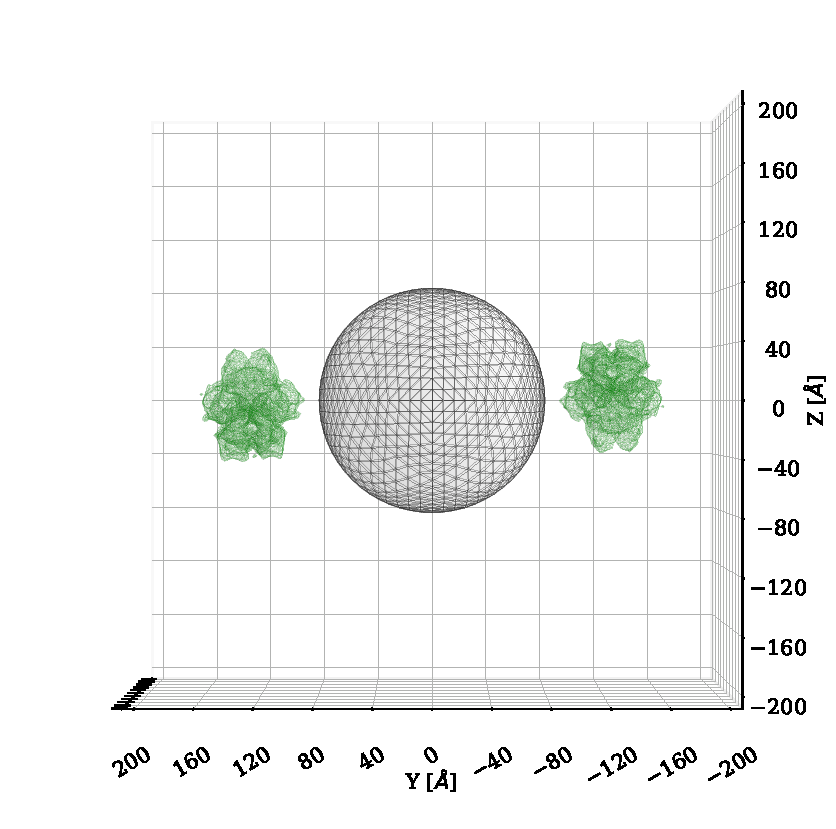
\includegraphics[width=0.65\textwidth]{2prot_1nm_y_R8nm.pdf}} 
%   \caption{Sensor protein display: BSA located at 1 nm of the nanoparticle in the
%            y-direction}
    \caption{Sensor protein display: BSA located at $\pm 1 \, nm$ of the nanoparticle in the
            x-direction (top) and y-direction (bottom)}
    \label{fig:display_xy}
\end{figure*}
